\documentclass[12pt]{article}

\usepackage{fullpage}
\usepackage{graphicx}
\usepackage{graphics}
\usepackage{mdwlist}


% christos: these look closer to NSF specs\dots
\setlength{\oddsidemargin}{0.0in}
\setlength{\evensidemargin}{0.0in}
\setlength{\textwidth}{6.5in}
\setlength{\headheight}{0.0in}
\setlength{\topmargin}{0.0in}
% \setlength{\textheight}{9.0in}
\setlength{\textheight}{9in}
\addtolength{\textheight}{-\topmargin}
\addtolength{\textheight}{-\headheight}
\addtolength{\textheight}{-\headsep}
\addtolength{\textheight}{-\footskip}



\begin{document}

\newcommand{\beq}{\begin{equation}}
\newcommand{\eeq}{\end{equation}}
\newcommand{\bit}{\begin{itemize*}}
\newcommand{\eit}{\end{itemize*}}
\newcommand{\goal}[1]{ {\noindent {$\Rightarrow$} \em {#1} } }
\newcommand{\hide}[1]{}
\newcommand{\comment}[1]{ {\footnotesize {#1} } }
\newtheorem{lemma}{Lemma}
\newtheorem{theorem}{Theorem}
\newtheorem{proof}{Proof}
\newtheorem{defn}{Definition}
\newtheorem{algo}{Algorithm}
\newtheorem{observation}{Observation}

\title{Phase3: The Final Report}


\author{ {\em Yangqingwei Shi} \\	   
	    {\tt yangqin1@andrew.cmu.edu}
	 \and
	 {\em Hao Jin} \\
	     {\tt haoj@andrew.cmu.edu}}
\maketitle

\section{Plan for activites}
    \label{sec:intro}
    % {\em
% \bit
% \item
% what is the problem
% \item
% what are the applications
% \eit
% }

%\bit
%    \item In T3, Hao will be mainly working on the optimizations through database-related techniques such as indexing and query optimization while Yangqingwei will look into possible modifications to the algorithms and metadata caching to further improve the overall performance.
%    \item In T4, Yangqingwei will be working on plotting and analysis of data retrieved from application of our implementation on various datasets, and Hao will be working on adding portability support to the code so that the cost is minimum when we want to move to a different dataset with different number of dimensions.
%    \item In T5, we will be working together on this task as this will be the heaviest one. Each of us will work on some of the datasets and try out different settings. Finally, we will be working together on any possible further optimizations and work on documentations of our findings.
%\eit
\paragraph{} Most real-life information can be expressed as multi-aspect data(tensors) and easily stored as tables in relational databases. As the scales of websites grow these years, the sizes of datasets are also growing rapidly,
thus breaking the assumption that all data should fit into memory. This change challenges the traditional practices for processing data, thus we want to explore ways to handle datasets that do not fit into memory of normal-sized machines.
For this project we tried the possibility of using Structured Query Language(SQL), a powerful language that is able to handle data that does not fit in memory while still enabling us to adopt the latest technologies from database
researches for faster computation on large multi-aspect data. Since SQL can run on any hardware as long as there exists a proper DBMS, a successful SQL implementation will enable us to perform efficient analysis of multi-aspect datasets
of any size on any machine.

\newpage
\section{Survey}
    \label{sec:survey}
    

\subsection{Papers read by Hao Jin}

The first paper was ``Graph Analytics using the Vertica Relational Database''.

\begin{itemize*}
\item {\em Problem Definition}: Many vertex-centric analyzers of graphs have been developed with the growing interest in graph processing in recent years. However, most of these systems were developed based on the assumption that new type of storage is used to store the data, which conflicts with the fact that most of graph datasets are still stored in traditional relational databases.

\item {\em Main idea}: To avoid the overhead of moving data around from traditional database to latest type of storage to perform graph analyses, this paper proposes that vertex-centric graph processing can be completed by database queries with proper change of the database system and the algorithm. With the switch to traditional databases, graph queries can also make use of the existing optimization techniques in current database systems. The paper analyzed the SQL implementation of Single Source Shortest Path(SSSP), CC(Connected Components), and PageRank together with corresponding query optimizations and system extensions. The optimizations range from optimizations on the queries themselves, to existing execution optimizations in Vertica system, to specialized extensions to Vertica for the graph tasks. The authors performed experiments on sample datasets to compare the performance of the same graph queries in different systems and showed that using Vertica can greatly reduce the memory footprint of typical vertex-centric queries while still achieve competitive performance on sample datasets compared with GraphLab and Giraph. Beyond these kinds of queries, Vertica also performed well on advanced graph analyses such as Strong Overlap and Weak Ties, while Giraph ran out of memory on those two test. In conclusion, the authors show that vertex-centric graph analyses, even the ones that can not be handled by existing graph analytics systems, can be implemented in SQL to take advantage of existing optimizations in DBMS and achieve competitive performance.
\item {\em Use for our project}:
      This paper is very useful for the project since it provides several approaches for rewriting traditional vertex-centric graph analyses to database SQL queries and also provides the necessary approaches for optimizing the queries for faster queries. 
\item {\em Shortcomings}:
      This paper’s experiment was performed on Vertica, which is a commercial DBMS product that provide many extra features and many optimizations than Postgres. Since we will be using Postgres for our project, we may not have access to some optimizations mentioned in this paper and will have to find alternative optimizations for the graph algorithms. On the other hand, the paper put emphasis on only 3 typical graph analysis workloads and mentioned 2 other types of graph analysis(Strong Overlap and Weak Ties) briefly. Since we may want to do comprehensive analysis on the datasets in our project, we’ll have to think about how to transform other graph analysis workloads to efficient database queries.
\end{itemize*}

\newpage
The second paper was ``GBASE: an efficient analysis platform for large graphs''
\begin{itemize*}
\item {\em Problem Definition}: With the increasing interest in data mining of graphs, there’s more and more effort put into efficient processing of computations on graphs. The sizes of target graphs can easily reach billion nodes and edges, thus occupying great amount of disk space and consuming much memory during computation. As a result, efficient storage, computation, and optimization become big problems for mining such graphs and need to be addressed effectively.\\

\item {\em Main idea}: The paper focuses on the implementation of a general-purpose graph analysis system, GBASE, to address the problems with processing large-scale graphs. The system improves the performance of a bunch of graph analysis algorithms on large-scale graphs through efficient storage methods to reduce cost of storage and cost of query, various fast algorithms for a wide range of graph queries for faster response to queries, and graph processing optimization techniques for efficient execution of queries. The proposed formulation, compression and placement methods of blocks are proven to compress the graph data greatly, thus reducing the storage consumption. For several typical graph queries, the paper gave the matrix-vector multiplication form of the queries together with detailed SQL implementations. Since matrix-vector multiplications can be parallelized for faster performance, the paper also provided the Hadoop algorithm and applicable optimizations for execution. The space efficiency achieved by the storage improvements and the boost in query processing resulted from better algorithm and optimized parallel execution are proven via experiments on different datasets. In conclusion, GBASE is a graph processing platform that provides the users with compression of graph data, efficient algorithms for typical graph queries and effective optimizations of executions.\\
\item {\em Use for our project}:
      This paper should be useful for our project. Firstly the detailed SQL implementations provided in the paper can serve as the building blocks of our final project. On the other hand, the reduction of graph query problems to matrix multiplications provide a very good idea of handling other types of graph queries, which may be useful when we get deeper into the project. Finally, the use of open-source parallel programming frameworks provide a good hint for optimization of computation components of the final project.\\
\item {\em Shortcomings}:
      The compression method is based on the assumption that the graph data is not updated because the formulation of blocks is based on partition of graphs, if we want to constantly update our graph for latest version of the data, then we need to repeat the formulation, compression, and placement again and again. On the other hand, more transformation from graph queries to SQL queries can be developed for advanced graph queries.
\end{itemize*}

\newpage
The third paper was ``PEGASUS: A Peta-Scale Graph Mining System - Implementation and Observations''
\begin{itemize*}
\item {\em Problem Definition}: Sizes of real graphs of interest are ever-growing. With the vast growth of web services, more and more graphs are reaching tera- or peta-byte in size. As a result, we need various analyses of those graph data to be quick enough for those analyses to be feasible for wider range of users.  Since all those different kinds of queries serve different purposes, it’s hard to find a common approach for improving the performance for each one of them.\\

\item {\em Main idea}: This paper is about the generalization of graph queries into matrix-vector multiplication and the corresponding implementations and optimizations of such generalization. The paper proposed the “Generalized Iterative Matrix-Vector multiplication”(GIM-V) model as the underlying primary computation for various kinds of graph queries. This model unifies many kinds of computations on graphs to the simpler computations of matrix-vector multiplications. Reductions from PageRank, Random Walk with Restart and Diameter Estimation to GIM-V model are shown in the paper as examples, and are proven to produce the correct results. Then the authors moves one to efficient implementation and execution of GIM-V model. The paper also analyzed the performance of this generalization and compared the effectivenesses of different optimizations in the paper on different types of queries through applying the model and different optimizations on datasets collected from real network services on M45 supercomputing cluster provided by Yahoo!. In conclusion, PEGASUS is a system for efficient graph mining of extreme-scale graphs that adopts GIM-V model as the common underlying primitive for a variety of graph queries. With proper combinations of optimization techniques, the system can perform fast analysis on peta-scale real graph data. With the help of HADOOP framework, the system can achieve portable parallelization of computation.\\
\item {\em Use for our project}:
      This paper is definitely useful for our project. It’s a further step from the GBASE paper on generalizing useful graph algorithms to matrix-vector multiplications, and it shows very good performance gains from this generalization. Moreover, suitable optimizations with proven performance for the model are also given in the paper, which will be useful for the large datasets we work on for this final project. The paper also mentioned that PEGASUS may be useful for tensor analysis on HADOOP, which fits the topic of the final project very well, so we may want to dig deeper in that direction.\\
\item {\em Shortcomings}:
      Only 3 kinds of graph queries are mentioned in the paper. However, there are many other graph queries that are necessary for our project, thus further effort should be invested in thinking about how to transform other types of graph queries to GIM-V model to take advantage of the features of the model.
\end{itemize*}



\subsection{Papers read by Yangqingwei Shi}

The fourth paper was ``A General Suspiciousness Metric for Dense Blocks
in Multimodal Data''

\begin{itemize*}
\item {\em Problem Definition}: A lot of data in our real life can be represented by multimodal data, we call it a tensor. In most cases, we want to find the suspicious dense block from a given tensor. However, until now there is even no specific criteria of the suspiciousness of a dense block. \\

\item {\em Main idea}: The main contribution of the paper can be devided into two parts. In the first part, the authors proposed a detailed mathematical model of multimodal dataset and dense blocks. In specific, it gives the definition of tensor $\chi$, subtensor $\gamma$, the mass $m$ and density $\rho$.The author also gives metric criteria of suspiciousness based on a list of five axioms. The five axioms are based on comparison of suspiciousness of two dense blocks. Derived from the five axioms, the author gave out a mathematical expression of suspiciousness of a dense block that is:

 \[f(n, c, N, C) = -log[Pr(Y_n = c)] \]
 
It is based on an Erd\"{o}s-R\'{e}nyi-Poisson model, and $Y_n$ is the number of entries. 
 
In the second part of the paper the author gave out a simple algorithms \textsc{CrossSpot} for finding suspicious blocks in a tensor and rank them in order. The algorithm start from a random seed and repeatedly adjust the dataset until it converges. The complexity of the algorithm is $O(T\times K\times (E + N log N))$, which is quasi-linear in $N$ and linear in the number of entries. \\

\item {\em Use for our project}:
      The main use of this paper is its first part, the model of dense blocks in multimodal data as well as the criteria of the suspiciousness of a dense block. The most useful part of this paper is the suspiciousness function. With suspiciousness function , we can quantify the suspiciousness into value so that we can easily evaluate the performance of our project. \\
      
\item {\em Shortcomings}:
      The \textsc{CrossSpot} algorithm is the weakest algorithm among all three algorithms, in comparison with \textsc{M-Zoom} and \textsc{D-Cube}. The local search may take a long time before it converges. Also, the algorithm start from a seed subtensor randomly, which I think might cause error. Although the authors confirmed there is no problem, the scale of the evaluation in the paper was not so sufficient.
\end{itemize*}

\newpage
The fifth paper was ``M-Zoom: Fast Dense-Block Detection in Tensors with Quality Guarantees''

\begin{itemize*}
\item {\em Problem Definition}: Finding dense blocks in a multimodal tensor has many applications in real world. In the former paper ``\textsc{CrossSpot}'', the definition and criteria  of data mining in tensor had been clear provided. However, all recent algorithms on dense block detection suffers from problems of flexibility, scalability, effectiveness. There is no algorithm having accuracy guarantees.\\

\item {\em Main idea}: The main contribution of the paper can be concluded to a better algortihm for dense block detection in tensors, called \textsc{M-Zoom}. In contrast to to other existing algorithms, \textsc{M-Zoom} has better performance, scalaibilty, effectiveness and accuracy. It slight changes the definition of traditional dense block terms by including the word relation $R$ which is a set of attributes and a measure attribute. The algorithm of \textsc{M-Zoom} repeatedly finding a single dense block on the remain relation, moving the block out of relation, and adding the block of the original relation including the exactly same attributes to list of dense blocks. The detection of single dense block is attribute-based. The attribute of the blocks are maintained by a priority queue or min-heap and moved out in order. A snapshot will record the density of the result after each movement and select the block of largest density. The effectiveness and the performance of \textsc{M-Zoom} is promised by this implementation. In each iteration of detecting single dense blocks, the algortihm provides a size bound and filter out all dense blocks that are not in the size bound. The accuracy is guaranteed by the size bound that the accuracy of the dense blocks within size bound is proved to be more accurate than those outside the bounds. The total complxity of the problem is near linear.\\

\item {\em Use for our project}:
      \textsc{M-Zoom} is a great algorithm with high performance and accuracy. I think it will be the algorithm we mainly based on in this project because it is effective and also simple. \textsc{D-Cube} algorithm has much higher performance in a distributed system. However, I think the data in our project is not very huge scale. As a result, we do not need a distributed system and \textsc{M-Zoom} will be the best option. \\
      
\item {\em Shortcomings or Suggestions}:
      This algorithm filter the block by size bounds. Actually, I think filtering out all results outside the bound is not practical. Sometimes, small size bound or large size bound data bay also represent a type of data. It might be helpful if we get them at the same time we doing data mining and evaluate them. On the other hand, the paper said the algorithm is scalable, but as the dimension of the if we maintain the same size bound, the result may have less accuracy promise. 
      
    
      
\end{itemize*}
\newpage
The sixth paper was ``D-Cube: Dense-Block Detection in Terabyte-Scale Tensors''

\begin{itemize*}
\item {\em Problem Definition}: While \textsc{M-Zoom} is a good algorithm in dense block detecting in tensors with accuracy guarantee and good performance, it has limitation that it cannot perform well on big data. In real world, the scale of data is increasingly huge. In most cases, these data are recorded in distributed systems. As a result, we need to optimize the \textsc{M-Zoom} algorithm to a new algorithm that make good use of distributed system.  \\

\item {\em Main idea}: The main contribution of the paper is an optimized \textsc{M-Zoom} algorithm on distributed system called \textsc{D-Cube}. Same as \textsc{M-Zoom}, \textsc{D-Cube} also have good scalabiility and accuracy guarantees. In contrast to to \textsc{M-Zoom}, \textsc{D-Cube} has an enhanced performance on distributed systems. In this paper, the author assumed the tuple data of tensor (single points) are distributed in a distributed file system. Briefly speaking, \textsc{D-cube} optimized \textsc{M-Zoom} by changing the detection of single dense blocks from attribute-based to tuple-based. By such change, we can get more accuracy dense blocks that has a subset on each attribute. Furthermore, tuple-based methods have better performance on distributed system. To prove this point, the paper also gave out an implementation of MapReduce method. In specific, the calculation of attribute now can be performed on distributed file systems as well as the filtering of tuples. As a result, \textsc{D-Cube} is a memory efficient algorithm on distributed system. \\

\item {\em Use for our project}:
      \textsc{D-Cube} has higher peroformance than \textsc{M-Zoom} on distributed systems. I think it will be an optional algorithm for our project. Since for small data, \textsc{M-Zoom} algorithm is sufficient. If we found our algorithm do not have good performance, we might change our algorithm to \textsc{D-Cube} and use it on a cloud platform. While on the other hand, the disk-based consideration of this paper is useful since we need implement our algorithm on another particular platform SQL. The consideration tells us that we need to understand SQL well before we simply copy the implementation onto it.\\ 
      
\item {\em Shortcomings}:
     I think \textit{M-Zoom} can also be implemented on distributed system because we can still distribute tuple data on a distributed file system. If this can be done, the contribution of \textsc{D-Cube} and the improvement will be not significant.
      
\end{itemize*}



	   
\newpage
\section{Implementation}
\subsection{Optimizations}
	\label{sec:imp}
	\subsubsection{Copy Method}
\paragraph{} The copy method implements line 8 of Algorithm 1(R=R-B) by making a copy of the previous table R with all tuples in B filtered out. We tested the performance of this method on one of the group member's laptop
using the workload of finding top 3 blocks from DARPA dataset with arithmetic density measure and select-by-density policy without any extra optimizations.
The computation took 1449 seconds to complete, and that will serve as the baseline performance for our SQL implementation and we'll compare the effect of optimizations to
this result.
\subsubsection{Mark Method}
\paragraph{} To implement the the mark method, we add an additional column on the R table named 'flag' and initialize all tuples with value 1 on the 'flag' column at the beginning. Then we implement line 8 of Algorithm 1(R=R-B) by
updating values of the 'flag' column to 0. The additional column caused some additional computations but the overall performance gets a boost after we adopt the mark method.
We tested the performance of this method on the same laptop with the copy method test using the same workload without any extra optimizations, the computation took 976 seconds to complete,
which is around 1.5 times speed-up compared to the baseline performance.
\subsubsection{Other Optimizations}
\paragraph{} We observed that the calculation of $M{\_}B(a,i)$ is very slow since we used a right join between B and B{\_}n to implement it, so we think that we’d better create indices on related tables in this join if we want to speed it up.
So we tried adding indices to the B{\_}n tables to improve the speed of this right join query. And we did achieve a significant speedup with indices on B{\_}n tables. This is tested on the same laptop used in the previous two sections.
Using copy method, with indices on B{\_}n, find top k = 3 blocks on darpa.csv, using arithmetic measure and select dimension by density policy: 306 seconds.
Using mark method, with indices on B{\_}n, find top k = 3 blocks on darpa.csv, using arithmetic measure and select dimension by density policy: 284 seconds.
Adding indices to B{\_}n gives us an overall speedup of around 3 compared to the results without those indices with the same method. So we can see that this optimization
is consistently boosting performance for both methods. So this means the calculation of $M{\_}B(a,i)$ is a bottleneck in our implementation and adding
indices to B{\_}n can improve the performance greatly.
\paragraph{} We also tried out adding indices to a bunch of other tables such as D{\_}n tables, however, it does not bring any
interesting performance boost that causes qualitative improvement to our performance.
\begin{table} [!ht]
\centering
\begin{tabular}{|c|c|c|c|}
    \hline
        Method & k & Time without extra indices & Time with extra indices \\
    \hline
        Copy & 3 & 1449 & 306\\
    \hline
        Mark & 3 & 976 & 284 \\
    \hline
\end{tabular}
\caption{Table of Benchmark Performance}

\end{table}

	
\newpage
\section{Experiments}
\subsection{Evaluation}
	\label{sec:expeval}
	\subsubsection{Results}
\paragraph{} The results first five blocks of the darpa and airforce are shown in the tables above.
\begin{table}
\centering
\begin{tabular}{|c|c|c|c|c|}
    \hline
        Dataset & k & Dimension & Mass & Density \\
    \hline
        Darpa & 1 & 2 X 1 X 47 & 278288 & 16697.3 \\
    \hline
        Darpa & 2 & 8 X 3 X 118 & 688245 & 16005.7 \\
    \hline
        Darpa & 3 & 2 X 1 X 44 & 230124 & 14688.8 \\
    \hline
        Darpa & 4 & 1 X 1 X 5 & 26371 & 11301.8 \\
    \hline
        Darpa & 5 & 2 X 1 X 18 & 77425 & 11060.7 \\
    \hline
\end{tabular}
\caption {Top 5 dense blocks for Darpa Dataset}
\end{table}

\begin{table}
\centering
\begin{tabular}{|c|c|c|c|c|}
    \hline
        Dataset & k & Dimension & Mass & Density \\
    \hline
        Airforce & 1 & 1x1x1x1x1x1x1 & 1930307 & 1930307 \\
    \hline
        Airforce & 2 & 1x1x1x2x1x2x2 & 2532845 & 421776.6 \\
    \hline
        Airforce & 3 & 3x4x3x3x1x58x21 & 554067 & 41704.0\\
    \hline
        Airforce & 4 & 3x4x3x13x4x67x35 & 493873 & 25691.3 \\
    \hline
        Airforce & 5 & 1x1x3x1x1x36x20 & 168929 & 18769.9 \\
    \hline
\end{tabular}
\caption {Top 5 dense blocks for Airforce Dataset}
\end{table}

\subsubsection{Suspiciousness Analysis}
By just taking a look at the cardinality of all dimensions of the detected blocks, we can decide that some of those blocks are
anomalies right away since their cardinalities on all dimensions are relatively small and they still have high mass. Such blocks
suggest that some small number of users are sending extremely high volume of network traffic over a short period of time, which is very
suspicious activity.
Then We looked at all tuples in the detected blocks and cross-checked with the labelled dataset and found that most of those tuples in
the detected blocks turn out to be labelled as various network attacks, which proves our idea stated before. We also calculated
the true positive rate and false positive rate of our detected tuples, and we found with small number of blocks detected(<20), the true
postive rate is way higher than the false positive rate, which means that we are hitting most anomalous tuples while avoiding hurting many
benign tuples.

\newpage
\subsubsection{ROC and AUC}
The ROC Curve and the AUC value are shown in Figure 1 and Figure 2.
\begin{figure}[!ht]
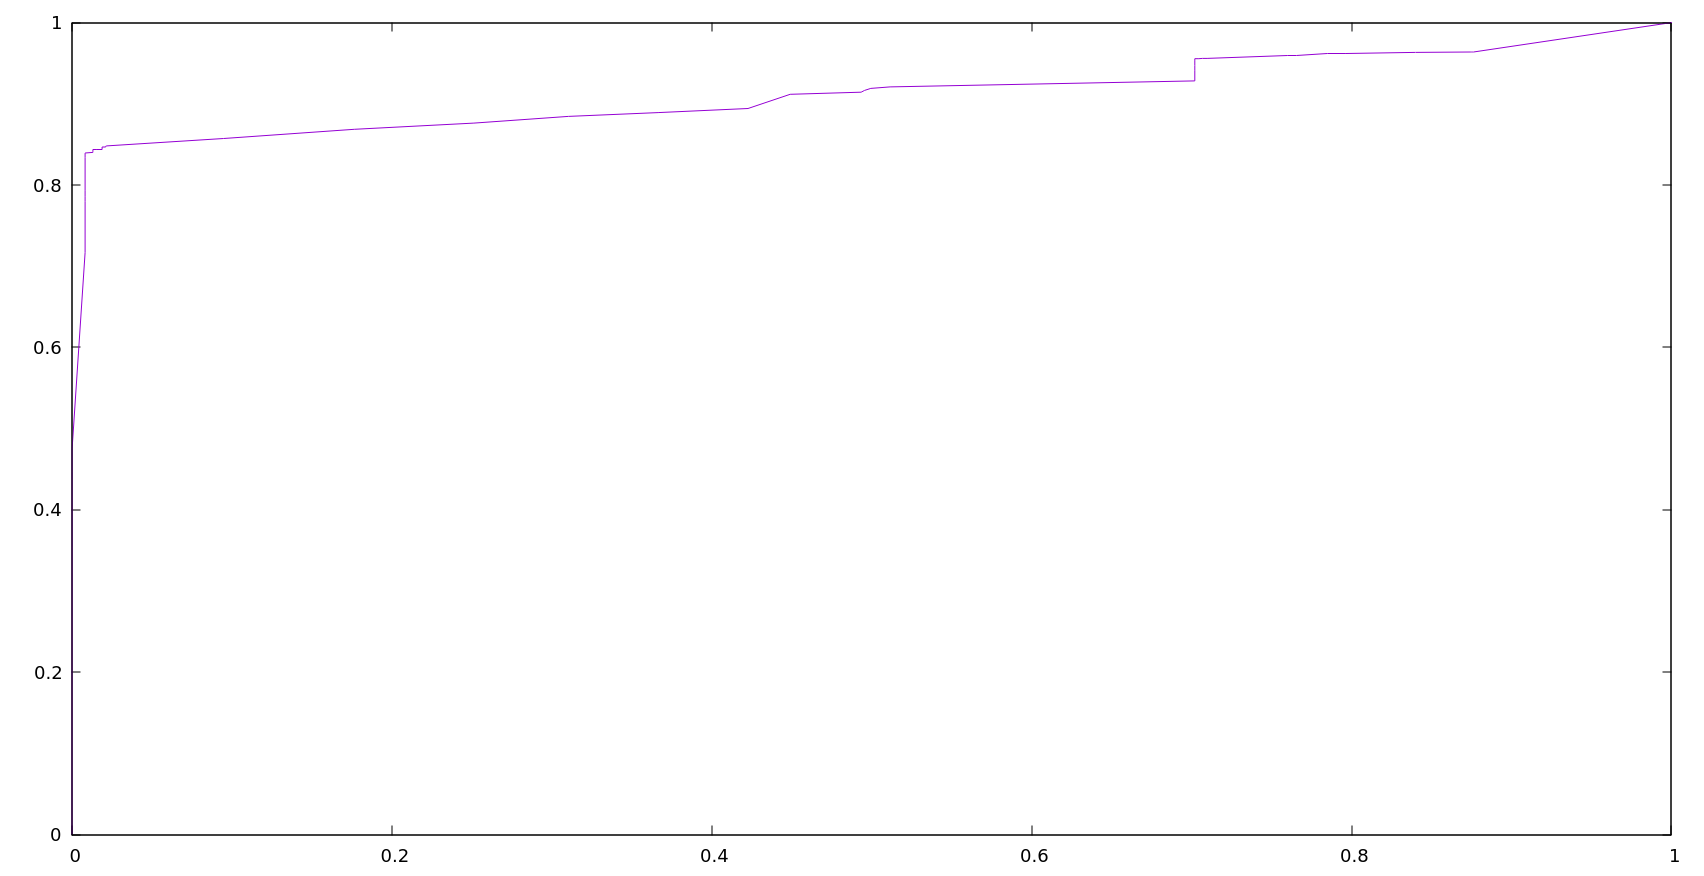
\includegraphics[scale=0.5]{roc1.png}
\caption{ROC Curve of Darpa Dataset After 60-Block Detections, AUC = 0.912}
\end{figure}

\begin{figure}[!ht]
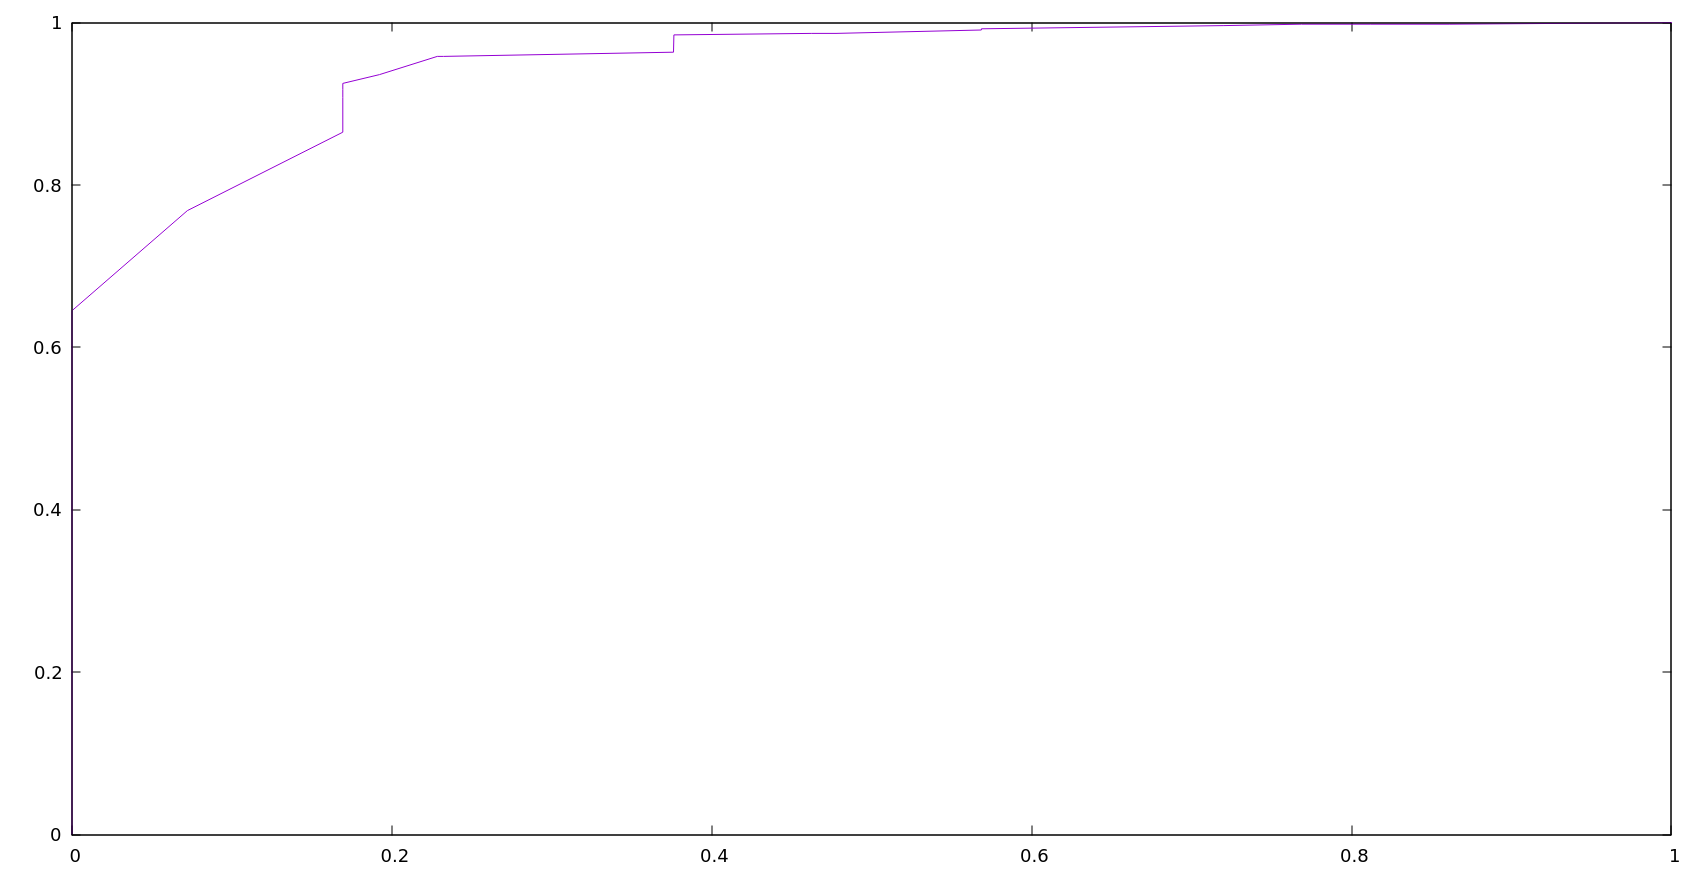
\includegraphics[scale=0.5]{roc2.png}
\caption{ROC Curve of Airforce Dataset After 20-Block Detections, AUC = 0.948}
\end{figure}
\paragraph{} From the ROC curves and AUC values we can see that the results we get on DARPA and AIRFORCE datasets are comparable to the
results presented in the original DCube paper. The true positive rate is way higher than false positive rate when number of blocks is small,
which means that our implementation can find the dense blocks which are most suspicious. The AUC values are also similar to the ones from the
original DCube paper. These results suggest that our SQL implementation can deliver results with comparable correctness on real-life datasets.

	
\subsection{Anomaly Detection}
	\label{sec:expanal}
	\subsection{Top 5 Blocks for Amazon, Wiki and Yelp Datasets}
\paragraph{}
\begin{table}
\centering
\begin{tabular}{|c|c|c|c|c|}
    \hline
        Dataset & k & Dimension & Mass & Density \\
    \hline
        Amazon & 1 & 60 x 60 x 1 x 1 & 3600 & 118.033 \\
    \hline
        Amazon & 2 & 150 x 150 x 3 x 2 & 7550 & 99.016 \\
    \hline
        Amazon & 3 & 40 x 40 x 1 x 1 & 1600 & 78.049 \\
    \hline
        Amazon & 4 & 35 x 35 x 1 x 1 & 1225 & 68.056 \\
    \hline
        Amazon & 5 & 3412 x 1745 x 1011 x 5 & 77694 & 50.344 \\
    \hline
\end{tabular}
\caption {Top 5 dense blocks for Amazon Dataset}
\end{table}
\begin{table}
\centering
\begin{tabular}{|c|c|c|c|c|}
    \hline
        Dataset & k & Dimension & Mass & Density \\
    \hline
        Wiki & 1 & 1 x 1 x 30 & 7756 & 2496.112 \\
    \hline
        Wiki & 2 & 3 x 3 x 744 & 16508 & 875.836 \\
    \hline
        Wiki & 3 & 1 x 1 x 22 & 1520 & 542.462 \\
    \hline
        Wiki & 4 & 13 x 11 x 730 & 22824 & 484.736 \\
    \hline
        Wiki & 5 & 75 x 35 x 744 & 40017 & 320.143 \\
    \hline
\end{tabular}
\caption {Top 5 dense blocks for Wiki Dataset}
\end{table}
\begin{table}
\centering
\begin{tabular}{|c|c|c|c|c|}
    \hline
        Dataset & k & Dimension & Mass & Density \\
    \hline
        Wiki & 1 & 60 X 60 X 1 X 1 & 3600 & 118.033 \\
    \hline
        Wiki & 2 & 55 X 55 X 1 X 1 & 3025 & 108.036 \\
    \hline
        Wiki & 3 & 50 X 50 X 1 X 1 & 2500 & 98.039 \\
    \hline
        Wiki & 4 & 45 X 45 X 1 X 1 & 2025 & 88.043 \\
    \hline
        Wiki & 5 & 5416 X 4464 X 2792 X 5 & 268578 & 84.745 \\
    \hline
\end{tabular}
\caption {Top 5 dense blocks for Yelp Dataset}
\end{table}
\subsection{Suspicious Blocks}
\paragraph{Amazon Dataset} We think that none of the top 5 blocks for Amazon dataset is a suspicious block. For the top 4 blocks, we can interpret them as some users gave the same rating to some different apps during the same hour, which is a
very possible event considering the number of users of Amazon and the granularity of the timestamp. For the last block among the top 5 blocks, we observe that the cardinality of the last dimension is 5, which equals to the cardinality of
that dimension of the original dataset, and it means that a lot users gave all kinds of ratings to a wide range of apps during a long time period, which is just normal behaviour of websites of Amazon's size.
So we think none of those blocks from Amazon dataset is an anomaly.
\paragraph{Wiki Dataset} We think that block 2 may be a dense block since this means that a small number of users updated a small number of pages a large number of times, thus we think block 2 may be an anomaly. All other blocks are either
small number of users making few changes to the same page or larger number of users make many changes to a wider range of pages, which, we think are legal activities for Wikipedia. So for Wiki dataset we think block 2 may be an anomaly.
\paragraph{Yelp Dataset} We think that none of the top 5 blocks for Yelp dataset is a suspicious block. For the top 4 blocks, we can interpret them as some users gave the same rating to some different businesses during the same hour, which is a
very possible event considering the number of users of Yelp and the granularity of the timestamp. For the last block among the top 5 blocks, we observe that the cardinality of the last dimension is 5, which equals to the cardinality of
that dimension of the original dataset, and it means that a lot users gave all kinds of ratings to a wide range of businesses during a long time period, which is just normal behaviour of websites of Yelp's scale.
So we think none of those dense blocks from Yelp dataset is an anomaly.


\newpage
\section{Conclusions}
	\label{sec:concl}
	\paragraph{} Firstly, we successfully completed the implementation of DCube dense block detection algorithm with proper optimizations. Although the overall performance of our implementation
using Postgres is still way slower than the original implementation of DCube, it is still acceptable considering the difference in the speed of hard disks and memory chips. What's more,
we compared the effects of different implementation details on overall performance and provided additional successful optimizations to further improve the performance of our detector.
\paragraph{} Secondly, the outputs of our dense block detector shows that our implementation can correctly detect the top dense blocks in real-life multi-aspect data. The ROC curve of
our results on DARPA and AIRFORCE datasets shows that we have a high true positive rate for detecting network attacks, and the AUC value also illustrates the correctness of our implementaion.
\paragraph{} Thirdly, we successfully extended the usage of our dense block detector to more real-life tensors and successfully detected the top dense blocks in those datasets and also gave our
insights on whether the dense blocks are anomalies or not.
\paragraph{} Furthermore, although we've proved that our implementation has good speed and correct results, there's always room for improvement, we think that this project can still be
improved in the following ways:
\begin{enumerate}
\item Use a different DBMS for even faster execution.
\item Create even more indices to improve as much of the computation as possible.
\item Application to more real-life data to check for correctness and performance.
\end{enumerate}



\bibliography{BIB/christosref,BIB/other}
\bibliographystyle{plain}


\newpage
\pagenumbering{roman}


\end{document}
